\documentclass{article}
\usepackage{graphicx} % Required for inserting images
\usepackage{subcaption}
\usepackage{minted}
\usepackage{float}
% \usepackage{listings}
\usepackage{amsmath}
\usepackage{amssymb}
% \usepackage{xcolor}
\title{Scientific Computation Project2}
\author{02242457}
\date{December 2024}

\begin{document}
\maketitle
\section{Part 1.}
\subsection{}

1.(a) Focusing on the non-trivial case where \( X_i \neq 0 \), we cancel \( X_i \) (as it is nonzero) from the equation, This gives a linear system of equations for the equilibrium values \( \{X_0, X_1, \dots, X_{n-1}\} \), which can be rewritten compactly as:

\[
1 - X_0 - \gamma(X_{n-2} + X_1) + \mu X_{n-3} = 0,
\]
\[
1 - X_1 - \gamma(X_{n-1} + X_2) = 0,
\]
\[
1 - X_i - \gamma(X_{i-2} + X_{i+1}) = 0, \quad \text{for } 2 \leq i \leq n-2,
\]
\[
1 - X_{n-1} - \gamma(X_{n-3} + X_0) = 0.
\]
The Jacobian matrix \( J \) is constructed to represent the linearized system of ODEs near the equilibrium point \( \bar{x} \). Each entry \( J[i,j] \) approximates the partial derivative \( \frac{\partial f_i}{\partial X_j} \).The matrix \( M = \exp(J \cdot T) \) is the matrix exponential of the Jacobian \( J \) scaled by time \( T \). By finding the eigenvalues and eigenvectors of \( M^T M \), the code identifies the dominant mode of growth, corresponding to the largest eigenvalue, which is \( \text{eratio} \).

1.(b) Design:The test function calls part1q1a to compute the predicted maximum perturbation energy ratio. Then the system's dynamics are simulated using \texttt{simulate1}, starting with an initial state 
\[
X_0 = \bar{x} + \epsilon \tilde{x}_0,
\]
where \( \epsilon \) is a small perturbation magnitude. The perturbation energy at \( t = 0 \) (\( e_0 \)) is calculated as the norm of \( \epsilon \tilde{x}_0 \):
\[
e_0 = \|\epsilon \tilde{x}_0\|^2,
\]
while the energy at \( t = T \) (\( e_T \)) is determined from the deviation of the final state from \( \bar{x} \):
\[
e_T = \|x(T) - \bar{x}\|^2.
\]
The simulated energy ratio is then given by:
\[
\text{eratio\_sim} = \frac{e_T}{e_0}.
\]
Result:
\[
\text{Perturbation energy ratio from part1q1a: } 26879.8944517675
\]
\[
\text{Perturbation energy ratio from simulation: } 26873.539939897364
\]
1.(c)
\begin{figure}[H]
     \centering
     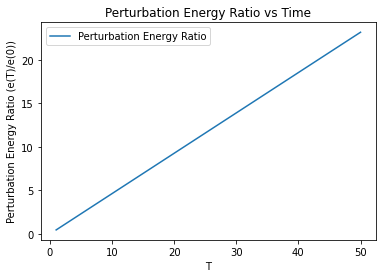
\includegraphics[width=0.75\linewidth]{part1_figure/Perturbation_T.png}
     \caption{perturbation energy vs time}
     \label{fig:GMRES vs iteration}
 \end{figure}
 The linear relationship between \( t \) and \( \log \left( \frac{e(t=T)}{e(t=0)} \right) \) arises because the perturbation energy grows exponentially over time, governed by the dominant eigenvalue \( \lambda_{\text{max}} \) of \( M^\top M \), where \( M = \exp(J \cdot T) \). The logarithm of the energy ratio, \( \log \left( \frac{e(t=T)}{e(t=0)} \right) \), is proportional to \( t \cdot \log(\lambda_{\text{max}}) \), resulting in a straight line.


\subsection{Question2}
\begin{figure}[H]
     \centering
     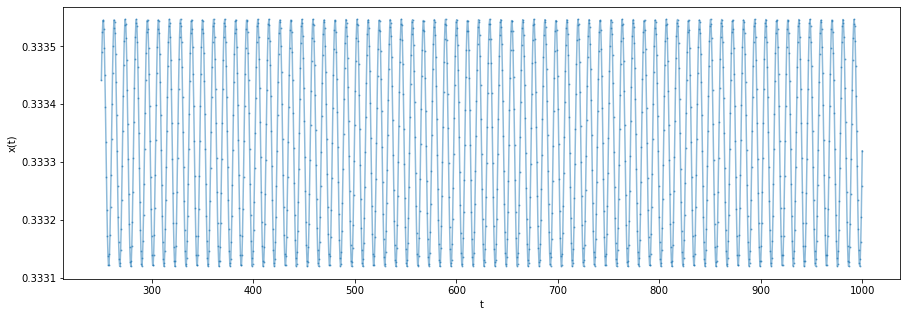
\includegraphics[width=0.75\linewidth]{part1_figure/part1_figure/n=9_timeseries.png}
     \caption{n=9 time series}
     \label{fig:GMRES vs iteration}
 \end{figure}
 
\begin{figure}[ht] % Placement options for the entire figure
     \centering
     \begin{subfigure}[b]{0.45\linewidth} % Width of subfigure
         \centering
         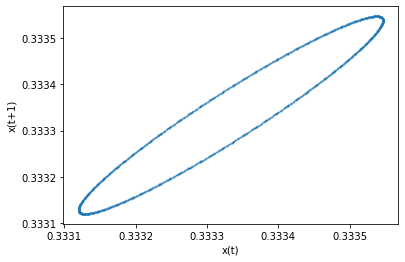
\includegraphics[width=\linewidth]{part1_figure/part1_figure/n=9_returnmap.png}
         \caption{Return Map for n=9}
         \label{fig:subfig1}
     \end{subfigure}
     \hfill
     \begin{subfigure}[b]{0.45\linewidth} 
         \centering
         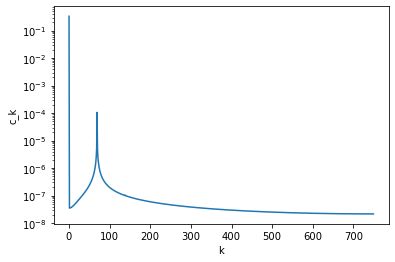
\includegraphics[width=\linewidth]{part1_figure/part1_figure/n=9_fourier.png}
         \caption{Fourier Coefficient for n=9}
         \label{fig:subfig2}
     \end{subfigure}
     % \caption{Overall caption for the figure}
     \label{fig:combined_fig}
%  \end{figure}
% \begin{figure}[ht] % Placement options for the entire figure
%      \centering
     \begin{subfigure}[b]{0.45\linewidth} % Width of subfigure
         \centering
         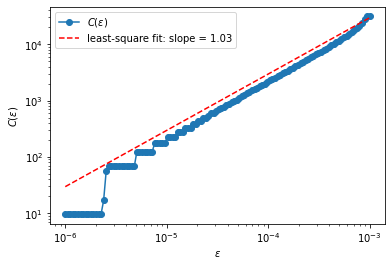
\includegraphics[width=\linewidth]{part1_figure/part1_figure/n=9_ce.png}
         \caption{Correlation Sum for n=9}
         \label{fig:subfig1}
     \end{subfigure}
     \hfill
     \begin{subfigure}[b]{0.45\linewidth} 
         \centering
         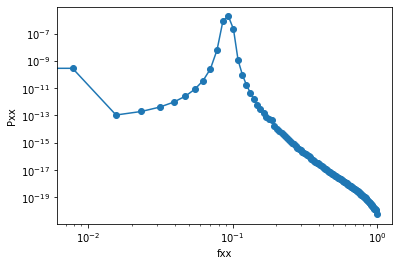
\includegraphics[width=\linewidth]{part1_figure/part1_figure/n=9psd.png}
         \caption{Power Spectral Density for n=9}
         \label{fig:subfig2}
     \end{subfigure}
     % \caption{Overall caption for the figure}
     \label{fig:combined_fig}
 \end{figure}
\textbf{When n=9}, the time series plot shows periodicity and the same amplitude every period. It indicates consistency and no chaos. The return map x (t) against x (t + 1) has a clear shape of an ellipse, suggesting periodic behavior.The width and height of the ellipse correspond to the amplitude of x in the time series plot. Fourier plot with a peak represents a dominant frequency. A strong single peak at a specific k indicates periodic behavior with a well-defined frequency, which is in agreement with previous analysis. The correlation dimension=1.03 suggests Low Dimensionality,corresponds to systems with a regular, one-dimensional trajectory.The PSD plot displays a distinct peak at the dominant frequency, indicating that the system has regular periodic oscillations.

\begin{figure}[H]
     \centering
     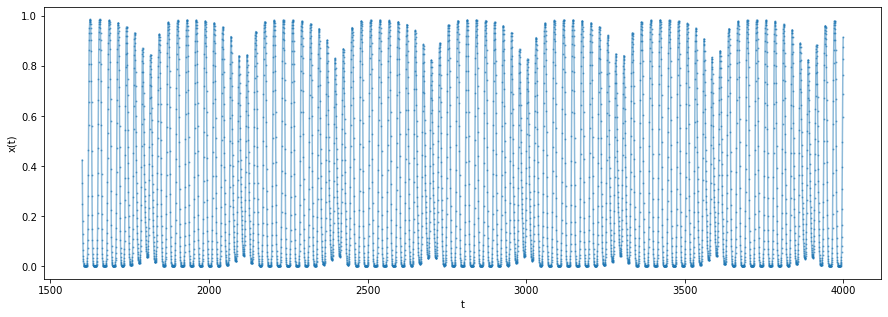
\includegraphics[width=0.75\linewidth]{part1_figure/part1_figure/n=20_timeseries.png}
     \caption{n=20 time series}
     \label{fig:GMRES vs iteration}
 \end{figure}
\begin{figure}[ht] % Placement options for the entire figure
     \centering
     \begin{subfigure}[b]{0.45\linewidth} % Width of subfigure
         \centering
         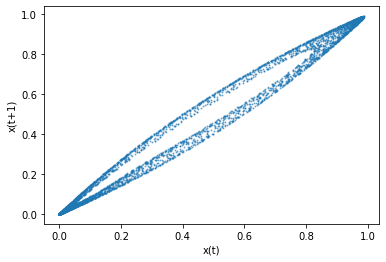
\includegraphics[width=\linewidth]{part1_figure/part1_figure/n=20returnmap.png}
         \caption{Return Map for n=20}
         \label{fig:subfig1}
     \end{subfigure}
     \hfill
     \begin{subfigure}[b]{0.45\linewidth} 
         \centering
         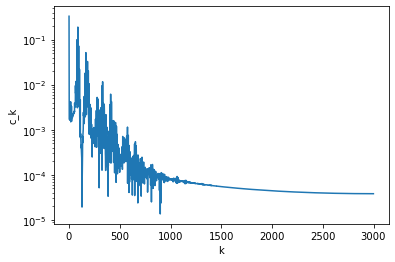
\includegraphics[width=\linewidth]{part1_figure/part1_figure/n=20fourier.png}
         \caption{Fourier Coefficient for n=20}
         \label{fig:subfig2}
     \end{subfigure}
     % \caption{Overall caption for the figure}
     \label{fig:combined_fig}
 % \end{figure}
 % \begin{figure}[ht] % Placement options for the entire figure
 %     \centering
     \begin{subfigure}[b]{0.45\linewidth} % Width of subfigure
         \centering
         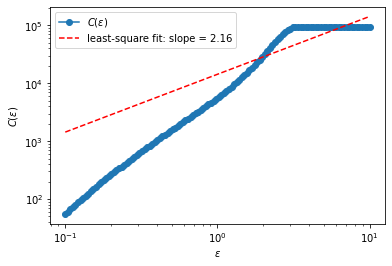
\includegraphics[width=\linewidth]{part1_figure/part1_figure/n=20ce.png}
         \caption{Correlation Sum for n=20}
         \label{fig:subfig1}
     \end{subfigure}
     \hfill
     \begin{subfigure}[b]{0.45\linewidth} 
         \centering
         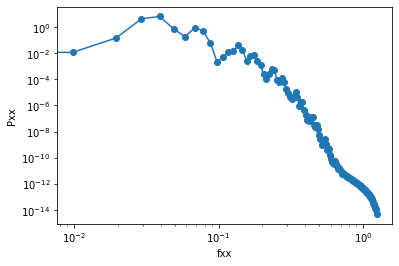
\includegraphics[width=\linewidth]{part1_figure/part1_figure/n=20psd.png}
         \caption{Power Spectral Density for n=20}
         \label{fig:subfig2}
     \end{subfigure}
     % \caption{Overall caption for the figure}
     \label{fig:combined_fig}
 \end{figure}
\textbf{When n=20}, in general it becomes more chaotic. The time series plot still shows periodicity, but the amplitude varies with t. This suggests the presence of a quasiperiodic signal, indicating a departure from the simple periodic dynamics observed before. The return map starts to have scatter points on the edge, but still has a fusiform shape with blank in the middle, indicating chaotic trajectories. The Fourier plot has multiple peaks, indicating quasiperiodicity. The correlation dimension of $D_c = 2.16$ is significantly higher than the $n = 9$ case ($D_c = 1.03$), indicating increased complexity in the dynamics. This value suggests the presence of a low-dimensional chaotic attractor. The fractional nature of the dimension implies that the system's trajectories are no longer confined to a simple one-dimensional manifold but instead explore a more complex, fractal-like phase space. The PSD plot shows multiple  peaks but less significant, suggesting that the system exhibits quasiperiodic with contributions from several frequencies.

\begin{figure}[H]
     \centering
     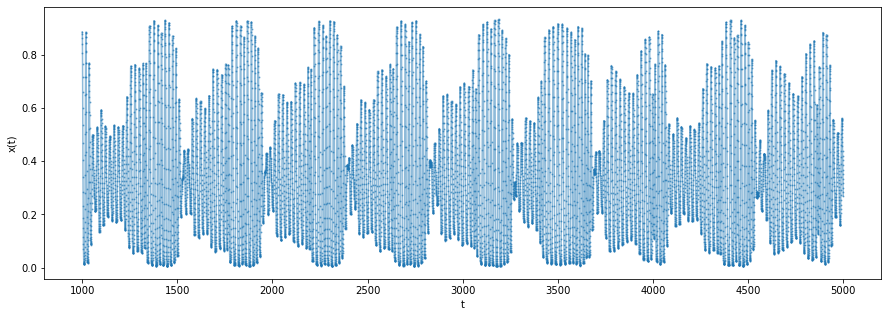
\includegraphics[width=0.75\linewidth]{part1_figure/part1_figure/n=59time.png}
     \caption{n=59 time series}
     \label{fig:GMRES vs iteration}
 \end{figure}
\begin{figure}[htp] % Placement options for the entire figure
     \centering
     \begin{subfigure}[b]{0.45\linewidth} % Width of subfigure
         \centering
         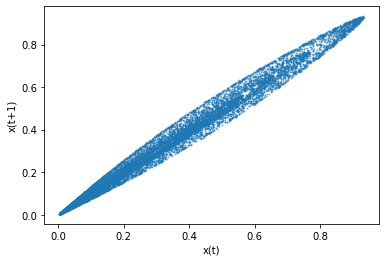
\includegraphics[width=\linewidth]{part1_figure/part1_figure/n=59return.png}
         \caption{Return Map for n=59}
         \label{fig:subfig1}
     \end{subfigure}
     \hfill
     \begin{subfigure}[b]{0.45\linewidth} 
         \centering
         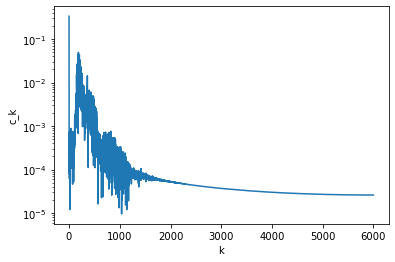
\includegraphics[width=\linewidth]{part1_figure/part1_figure/n=59fourier.png}
         \caption{Fourier Coefficient for n=59}
         \label{fig:subfig2}
     \end{subfigure}
     % \caption{Overall caption for the figure}
     \label{fig:combined_fig}
 % \end{figure}
 % \begin{figure}[ht] % Placement options for the entire figure
 %     \centering
     \begin{subfigure}[b]{0.45\linewidth} % Width of subfigure
         \centering
         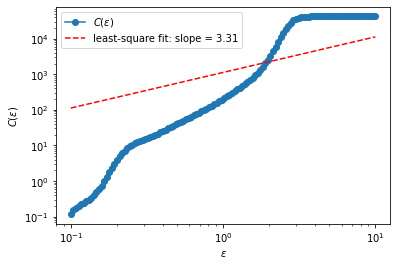
\includegraphics[width=\linewidth]{part1_figure/part1_figure/n=59ce.png}
         \caption{Correlation Sum for n=59}
         \label{fig:subfig1}
     \end{subfigure}
     \hfill
     \begin{subfigure}[b]{0.45\linewidth} 
         \centering
         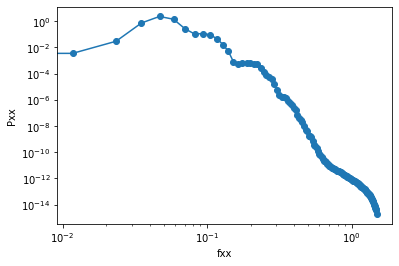
\includegraphics[width=\linewidth]{part1_figure/part1_figure/n=59_psd.png}
         \caption{Power Spectral Density for n=59}
         \label{fig:subfig2}
     \end{subfigure}
     \caption{Overall caption for the figure}
     \label{fig:combined_fig}
 \end{figure}
 \textbf{When $n = 59$}, the system exhibits strong chaotic behavior, as seen from the irregular time series, scattered return map, and broadband Fourier spectrum. The time series has more different amplitudes. The return map no longer has a clear edge and blank interior. The absence of periodic or quasiperiodic patterns highlights the transition to high-dimensional chaos. The correlation dimension of $D_c = 3.31$ confirms increased complexity, with the system exploring a fractal-like chaotic attractor in a higher-dimensional phase space. This behavior represents a significant departure from the simpler dynamics observed for $n = 9$ and $n = 20$. The PSD curve becomes smoother with no obvious peaks, showing a more mixed frequencies.
 
\section{Part 2.}
\subsection{Question1}
The \texttt{part2q1} function computes the first and second derivatives of a 2D array \texttt{f} with respect to \(x\) using an implicit finite difference method. It handles both interior and boundary points separately. For each row in the array, the method constructs a sparse system of equations based on finite difference coefficients. Special coefficients are used for the boundaries, while standard coefficients are applied for interior points. The system is solved using a sparse solver (\texttt{spsolve}), and the first and second derivatives are stored in \texttt{df} and \texttt{d2f} arrays, which are returned as output. This approach is efficient due to the use of sparse matrices and optimized solvers, reducing memory usage.

\subsection{Question2}
\begin{figure}[htp]
     \centering
     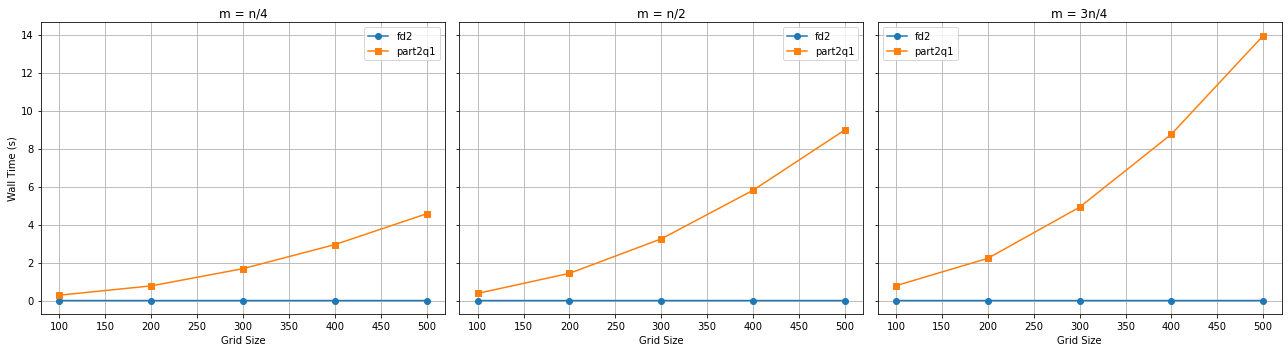
\includegraphics[width=1.1\linewidth]{part1_figure/Q2_figure/part2_figure/running_time_comparison3.png}
     \caption{running time against grid size for different m}
 \end{figure}
 This figure plots the running time agianst grid size using both methods(fd2 and part2q1) under sin(x). fd2 is quicker compared to part2q1 in all three cases. Here we change m (comparable to n) from m=n/4,n/2 and 3n/4. With larger m, the part2q1 diverges further from fd2 with grid size growing. Because when m becomes large, b(the RHS) becomes larger, requesting more matrix computation, leading to more running time. We'll descuss their accuracy below using two examples.
 
\begin{figure}[h] % Placement options for the entire figure
     \centering
     \begin{subfigure}[b]{0.48\linewidth} % Width of subfigure
         \centering
         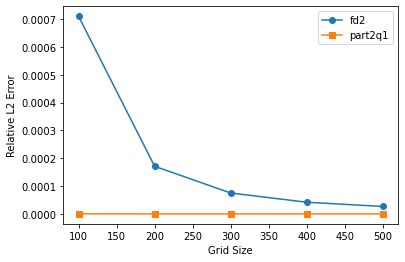
\includegraphics[width=\linewidth]{part1_figure/Q2_figure/part2_figure/errorplot1.png}
         \caption{error against grid size}
         \label{fig:subfig1}
     \end{subfigure}
     \hfill
     \begin{subfigure}[b]{0.45\linewidth} 
         \centering
         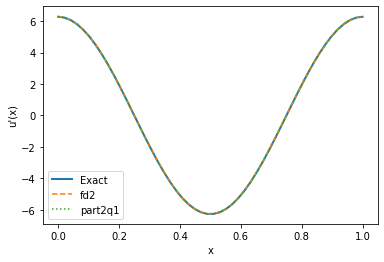
\includegraphics[width=\linewidth]{part1_figure/Q2_figure/part2_figure/functionplot1.png}
         \caption{First derivative plot when n=50 }
         \label{fig:subfig2}
     \end{subfigure}
     % \vspace{-5pt}
     \caption{test $\sin(2 \pi x)$}
     % \vspace{-10pt}
     \label{fig:combined_fig}
 \end{figure}
In the first derivative comparision plot, the three lines overlap, indicating both fd2 and part2q1 give the correct pattern, anlign with the exact solution. However in the error comparision plot, the fd2 has relative large error at small grid size and converge down when grid size increase, while the part2q1 remians low error at all time.\\
\\
\begin{figure}[htp] % Placement options for the entire figure
     \centering
     \begin{subfigure}[b]{0.45\linewidth} % Width of subfigure
         \centering
         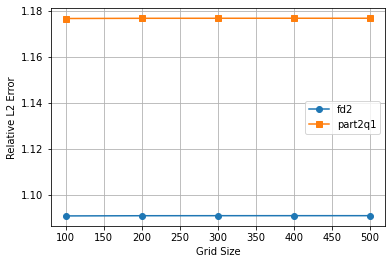
\includegraphics[width=\linewidth]{part1_figure/Q2_figure/part2_figure/errorplot2.png}
         \caption{error against grid size}
         \label{fig:subfig1}
     \end{subfigure}
     \hfill
     \begin{subfigure}[b]{0.45\linewidth} 
         \centering
         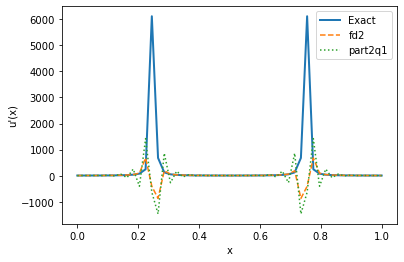
\includegraphics[width=\linewidth]{part1_figure/Q2_figure/part2_figure/functionplot2.png}
         \caption{First derivative plot when n=50}
         \label{fig:subfig2}
     \end{subfigure}
     \caption{test $\tan(2 \pi x)$}
     \label{fig:combined_fig}
 \end{figure}
\\
 Now we use the test function as $\tan(2 \pi x)$, with the singularity at boundaries.In the first derivative comparison plot, the three lines overlap at first and diverge at bountries. Both fd2 and part2q1 are opposite to the exact solution, suggesting that they fail to perform well at asymptotes. The error comparison plot shows the error of fd2 is less than part2q1 and both of them remain the same error with grid size varing.
when m becomes large, b(the RHS) becomes larger, requesting more loops in 
\end{document}



% \begin{figure}[H]
%     \centering
%     \includegraphics[width=0.75\linewidth]{GMRES_IT.png}
%     \caption{GMRES residual norm vs iteration}
%     \label{fig:GMRES vs iteration}
% \end{figure}


% \begin{figure}[ht] % Placement options for the entire figure
%     \centering
%     \begin{subfigure}[b]{0.45\linewidth} % Width of subfigure
%         \centering
%         \includegraphics[width=\linewidth]{GS_IT.png}
%         \caption{GS residual norm vs iteration}
%         \label{fig:subfig1}
%     \end{subfigure}
%     \hfill
%     \begin{subfigure}[b]{0.45\linewidth} % Width of subfigure
%         \centering
%         \includegraphics[width=\linewidth]{Jacobi_IT.png}
%         \caption{Jacobi residual norm vs iteration}
%         \label{fig:subfig2}
%     \end{subfigure}
%     \caption{Overall caption for the figure}
%     \label{fig:combined_fig}
% \end{figure}


